\section{Regressão Não-Linear}

Nestes problemas, nós vamos novamente aplicar Regressão Linear para classificação. Considere a função target

$$f(x_1,x_2) = sign(x_1^2 + x_2^2 - 0.6) $$

Gere um conjunto de treinamento de $N = 1000$ pontos em $\mathcal{X} = [-1, 1] \times [-1, 1]$ com probabilidade uniforme escolhendo cada $x \in \mathcal{X}$. Gere um ruído simulado selecionando aleatoriamente 10\% do conjunto de treinamento e invertendo o rótulo dos pontos selecionados.

newline \par
\textbf{Implementação:}

Para responder os itens referentes a este problema, foram implementado em Python duas classes: uma para gerar a função target não-linear (código \ref{cod:target_naolin}) e outra para gerar o Classificador Não-Linear (código \ref{cod:reg_naolin}). 

\begin{lstlisting}[language=Python, caption=Target Não-Linear, label=cod:target_naolin]
    # Classe para criar a função target não linear
    class TargetNaoLinear:
    
        # Método para classificar pontos de acordo a função target
        def classify_point(self, point): 
            return np.sign(point[0]**2 + point[1]**2 - 0.6)
        
        # Método para criar uma elipse para plots
        def criar_elipse(self):
            r = np.sqrt(0.6)
            elipse =  Ellipse(xy=(0,0), width=2*r, height=2*r, angle=np.degrees(0),
                               edgecolor='k', fc='None', lw=2, label='Função Target (f)')
            return elipse
\end{lstlisting}

A classe para gerar a função target não-linear possui dois métodos: um para classificar os pontos de acordo com $f(x_1,x_2) = sign(x_1^2 + x_2^2 - 0.6) $ e outro que gera uma elipse a partir $f(x_1,x_2)$ para ser plotada. Esta classe poderia ter sido quebrada em duas funções, porém foi decidido criar uma classe para agrupar as duas funções e também para que ela continuasse funcionando como entrada para o método $generate\_dataset(target)$ da classe $Dataset$ (código \ref{cod:dataset}), reaproveitada neste problema para gerar a base de dados $\mathcal{X}$.

\begin{lstlisting}[language=Python, caption=Classificador por Regressão Não-Linear, label=cod:reg_naolin]
    # Classe para criar e treinar o classificador linear
    class NaoLinear(Linear, w = np.zeros(6)):
        def __init__(self):
            self.w = w  # inicializa os pesos (incluindo o w_0)
        
        # Modifica o método para calcular a matriz X
        def calc_matriz_X(self, data):
            X = list()
            for point in data:
                x1 = point[0]
                x2 = point[1]
                X.append([1, x1, x2, x1*x2, x1**2, x2**2])
            return np.array(X)
        
        # Método novo para criar uma elipse para plots
        def criar_elipse(self):
            # Coeficientes da equação geral da cônica (Ax1^2 + Bx1x2 + Cx2^2 + Dx1 + Ex2 + F=0)
            # relacionados com os pesos (1, x1, x2, x1x2, x1^2, x2^2)
            A = self.w[4] # coef de x1^2
            B = self.w[3] # coef de x1x2
            C = self.w[5] # coef de x2^2
            D = self.w[1] # coef de x1
            E = self.w[2] # coef de x2
            F = self.w[0] # termo independente
            # Matrizes associadas à equação geral da cônica
            M = np.array([[A, B / 2], [B / 2, C]])
            offset = np.array([D, E])
            # Calcular o centro da elipse
            center = np.linalg.solve(-2 * M, offset)
            # Calcular os semi-eixos e o ângulo de rotação
            eigenvalues, eigenvectors = np.linalg.eigh(M)
            order = np.argsort(eigenvalues)
            eigenvalues = eigenvalues[order]
            eigenvectors = eigenvectors[:, order]
            semi_major = np.sqrt(-F / (eigenvalues[0] * eigenvalues[1])) / np.sqrt(eigenvalues[0])
            semi_minor = np.sqrt(-F / (eigenvalues[0] * eigenvalues[1])) / np.sqrt(eigenvalues[1])
            angle = np.arctan2(eigenvectors[1, 0], eigenvectors[0, 0])
            # Criar a elipse
            elipse =  Ellipse(xy=center, width=2 * semi_major, height=2 * semi_minor, angle=np.degrees(angle),
                            edgecolor='g', fc='None', lw=2, label='Hipótese (g)')
            return elipse
\end{lstlisting}

A classe do Classificador Não-Linear herda a classe do Classificador Linear (código \ref{cod:reglin}), modifica a inicialização dos pesos e o método para gerar a matriz de entradas $X$ seguindo o vetor de atributos não-linear $(1, x_1, x_2, x_1x_2, x_1^2, x_2^2)$ e insere um novo método que gera uma elipse a partir pesos calculados (relacionando eles com a fórmula geral das cônicas) para ser plotada.

Para testar as classes foram criadas duas funções: uma para plotar o dataset não-linear juntamente com a função target e a hipotese (código \ref{cod:scatterplot_nao_linear}), e outra parar gerar os dados utilizando a função target não-linear e ainda gerando ruido em 10\% deles e depois treinar um Classificador Não-Linear (código \ref{cod:teste_nao_linear}).

\begin{lstlisting}[language=Python, caption=Scatterplot Não-Linear, label=cod:scatterplot_nao_linear]
    def scatterplot_nao_linear(data, labels, target, hipotese):
        fig, ax = plt.subplots(subplot_kw={'aspect': 'equal'}, figsize=(8, 6))
        # plotar a função target
        elipse_target = target.criar_elipse()
        ax.add_patch(elipse_target)
        # plotar a hipótese
        if type(hipotese) is NaoLinear:
            elipse_hipotese = hipotese.criar_elipse()
            ax.add_patch(elipse_hipotese)
        elif type(hipotese) is Linear:
            w = hipotese.w
            x = np.linspace(-1, 1, 100)
            y_g = -(w[1] * x + w[0]) / w[2]
            plt.plot(x, y_g, 'g-', label='Hipótese (g)')
        else:
            return print("Hipotese não suportada")
        # plotar os pontos
        x_pos = [data[i][0] for i in range(len(data)) if labels[i] == 1]
        y_pos = [data[i][1] for i in range(len(data)) if labels[i] == 1]
        x_neg = [data[i][0] for i in range(len(data)) if labels[i] == -1]
        y_neg = [data[i][1] for i in range(len(data)) if labels[i] == -1]
        plt.scatter(x_pos, y_pos, c='blue', label='+1')
        plt.scatter(x_neg, y_neg, c='red', label='-1')
        # ajustar a figura       
        plt.xlim(-1, 1)
        plt.ylim(-1, 1)
        plt.xlabel('x')
        plt.ylabel('y')
        plt.title('Base de dados com a Função Target (f) não linear e Hipótese (g)')
        plt.legend(bbox_to_anchor=(1.05, 1), loc='upper left')
        plt.tight_layout(rect=[0, 0, 1, 1])
        plt.grid(True)
        plt.show()
\end{lstlisting}

\begin{lstlisting}[language=Python, caption=Teste para a Regressão Não-Linear, label=cod:teste_nao_linear]
    def teste(num_points, hipotese):
        # Criar a target não-linear
        target = TargetNaoLinear()
        # Criar o dataset
        dataset = Dataset(num_points)
        data, labels = dataset.generate_dataset(target)
        # Adicionar ruido
        selected_indices = np.random.choice(len(labels), int(len(labels) * 0.1), replace=False) # seleciona 10%
        labels[selected_indices] *= -1 # inverte o valor de 10%
        # Criar o classificador
        hipotese.fit(data, labels)
        # Plotar
        scatterplot_nao_linear(data, labels, target, hipotese)
\end{lstlisting}

O resultado da função $teste(num\_points, hipotese)$ para uma hipótese gerada pelo treinamento de uma Regressão Não-Linear pode ser observado na figura \ref{fig:naolinear_naolinear}.

\begin{figure}[H]
    \caption{Base de dados com a Função Target $(f)$ Não-Linear e a Hipótese $(g)$ Não-Linear}
       \centering
       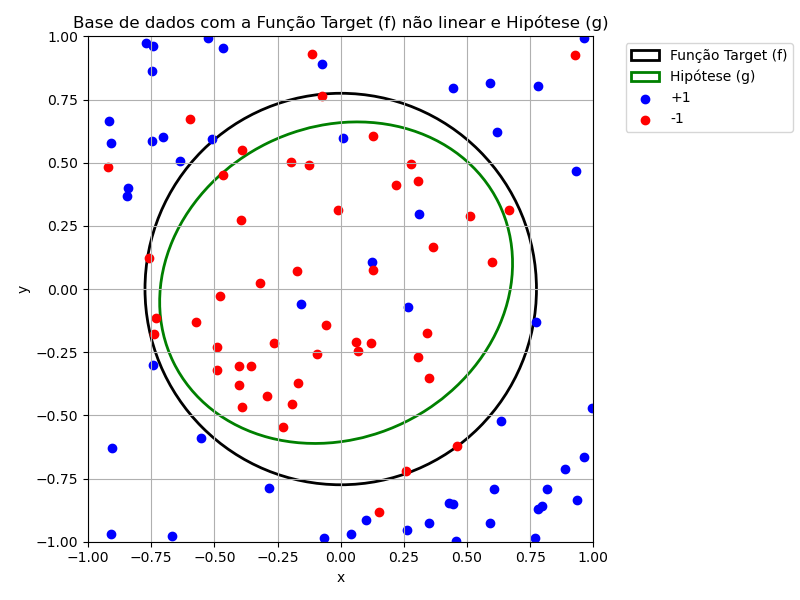
\includegraphics[width=12cm]{naolinear_naolinear.png}
       \label{fig:naolinear_naolinear}
\end{figure}

\begin{enumerate}
    \item Execute a Regressão Linear sem nenhuma transformação, usando o vetor de atributos $(1, x_1, x_2)$ para encontrar o peso $\boldsymbol{w}$. Qual é o valor aproximado de classificação do erro médio dentro da amostra $E_{in}$ (medido ao longo de 1000 execuções)?
    
    \begin{enumerate}
        \item 0
        \item 0.1
        \item 0.3
        \item [\textcolor{red}{(d)}]\textcolor{red}{0.5}\addtocounter{enumii}{1}
        \item 0.8
    \end{enumerate}
    
    \par

    \textbf{Justificativa:}

    Para responder a esse item foi implementada a seguinte função:

    \begin{lstlisting}[language=Python, caption=Cálculo do E\_in para a Regressão Linear, label=cod:calc_E_in_linear]
        def calc_Ein_linear(num_points, verbose = True):
            lista_E_in = list()
            for _ in range(1000):
                # Criar a target não-linear
                target = TargetNaoLinear()
                # Criar o dataset
                dataset = Dataset(num_points)
                data, labels = dataset.generate_dataset(target)
                # Adicionar ruido
                selected_indices = np.random.choice(len(labels), int(len(labels) * 0.1), replace=False) # seleciona 10%
                labels[selected_indices] *= -1 # inverte o valor de 10%
                # Criar o classificador não-linear
                linear = Linear()
                linear.fit(data, labels)
                # Classificar os pontos
                y_predicted = linear.classificar(data)
                # Calcular E_in para essa execução
                lista_E_in.append(np.mean(labels != y_predicted))
            E_in = np.mean(lista_E_in)
            # Plotar a última execução
            if verbose: print(f"E_in = {E_in:.4f}")
            return E_in
    \end{lstlisting}

    Foram realizadas 1000 execuções e em cada uma foi gerado um novo dataset para a função target $f(x_1,x_2) = sign(x_1^2 + x_2^2 - 0.6) $ e foi treinado um novo Classificador Linear. O $E_{in}$ em cada iteração foi calculado pelo número de erros dividido pela quantidade de pontos dentro da amostra. O valor final $E_{in} = 0.5044 = 50.44\%$ foi dado pela média dos $E_{in}$ em cada iteração. O valor de $E_{in}$ foi consideravelmente alto, como esperado de um Classificador Linear tentando classificar um dataset que não é linear. Como $0.5044$ está mais próximo de $0.5$ do que de $0.8$, o \textcolor{red}{item (d)} foi o escolhido.

    A figura \ref{fig:naolinear_linear} (gerada para apenas 100 pontos) ilustra por que o resultado do Regressor Linear foi tão ruim.

    \begin{figure}[H]
        \caption{Base de dados com a Função Target $(f)$ Não-Linear e a Hipótese $(g)$ Linear}
           \centering
           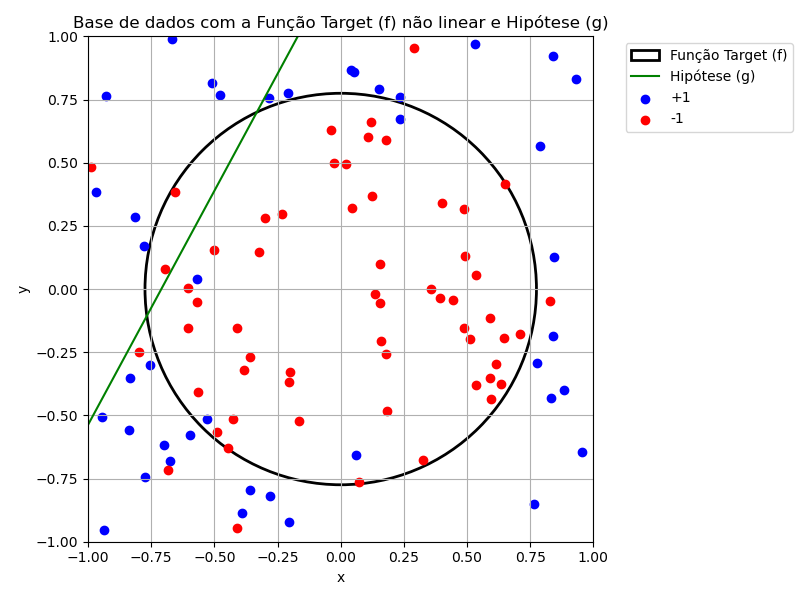
\includegraphics[width=12cm]{naolinear_linear.png}
           \label{fig:naolinear_linear}
    \end{figure}
    
    \item Agora, transforme os $N = 1000$ dados de treinamento seguindo o vetor de atributos não-linear $(1, x_1, x_2, x_1x_2, x_1^2, x_2^2)$. Encontre o vetor $\tilde{\boldsymbol{w}}$ que corresponda à solução da Regressão Linear. Quais das hipóteses a seguir é a mais próxima à que você encontrou? Avalie o resultado médio obtido após 1000 execuções.
    
    \begin{enumerate}
        \item [\textcolor{red}{(a)}]\textcolor{red}{$g(x_1,x_2) = sign(-1-0.05x_1+0.08x_2+0.13x_1x_2+1.5x_1^2+1.5x_2^2)$}\addtocounter{enumii}{1} 
        \item $g(x_1,x_2) = sign(-1-0.05x_1+0.08x_2+0.13x_1x_2+1.5x_1^2+15x_2^2)$
        \item $g(x_1,x_2) = sign(-1-0.05x_1+0.08x_2+0.13x_1x_2+15x_1^2+1.5x_2^2)$
        \item $g(x_1,x_2) = sign(-1-1.5x_1+0.08x_2+0.13x_1x_2+0.05x_1^2+0.05x_2^2)$
        \item $g(x_1,x_2) = sign(-1-0.05x_1+0.08x_2+1.5x_1x_2+0.15x_1^2+0.15x_2^2)$
    \end{enumerate}

    \par

    \textbf{Justificativa:}

    Para responder a esse item foi implementada a seguinte função:

    \begin{lstlisting}[language=Python, caption=Cálculo dos pesos para a Regressão Não-Linear, label=cod:calc_w_naolinear]
        def calc_w_naolinear(num_points, verbose = True):
            lista_w = list()
            for _ in range(1000):
                # Criar a target não-linear
                target = TargetNaoLinear()
                # Criar o dataset
                dataset = Dataset(num_points)
                data, labels = dataset.generate_dataset(target)
                # Adicionar ruido
                selected_indices = np.random.choice(len(labels), int(len(labels) * 0.1), replace=False) # seleciona 10%
                labels[selected_indices] *= -1 # inverte o valor de 10%
                # Criar o classificador não-linear
                naolinear = NaoLinear()
                w = naolinear.fit(data, labels)
                # Armazenar os pesos
                lista_w.append(w)
            w = np.mean(lista_w, axis=0)
            if verbose: 
                np.set_printoptions(suppress=True)
                print(f"w = {w}")
            return w
    \end{lstlisting}

    Foram realizadas 1000 execuções e em cada uma foi gerado um novo dataset para a função target $f(x_1,x_2) = sign(x_1^2 + x_2^2 - 0.6) $ e foi treinado um novo Classificador Não-Linear. O vetor $\boldsymbol{w}$ em cada iteração foi calculado pelo método $fit$ que multiplica a pseudo-inversa da matriz $X$ pelo vetor de labels. O valor final do vetor
     $$\tilde{\boldsymbol{w}} = [-0.9894, \quad -0.00164, \quad   0.0009, \quad   0.0031, \quad    1.5505, \quad   1.556]$$
      foi dado pela média em cada coluna da matriz $lista\_w$, a qual cada linha é composta pelo $\boldsymbol{w}$ calculado pelo treinamento naquela execução. O segundo, terceiro e quarto elementos divergem bastante das alternativas apresentadas, mas como o primeiro, o quinto e o sexto elementos se aproximam dos coeficientes da primeira alternativa, o \textcolor{red}{item (a)} foi o escolhido.
    
    \item Qual o valor mais próximo do erro de classificação fora da amostra $E_{out}$ de sua hipótese na questão anterior? (Estime-o gerando um novo conjunto de 1000 pontos e usando 1000 execuções diferentes, como antes).
    
    \begin{enumerate}
        \item [\textcolor{red}{(a)}]\textcolor{red}{0}\addtocounter{enumii}{1}
        \item 0.1
        \item 0.3
        \item 0.5
        \item 0.8
    \end{enumerate}

    Para responder a esse item foi implementada a seguinte função:

    \begin{lstlisting}[language=Python, caption=Cálculo do E\_out para a Regressão Não-Linear, label=cod:calc_E_out_naolinear]
        def calc_Eout_naolinear(num_points, w, verbose = True):
            lista_E_out = list()
            for _ in range(1000):
                # Criar a target não-linear
                target = TargetNaoLinear()
                # Criar o dataset de teste
                dataset = Dataset(num_points)
                data, labels = dataset.generate_dataset(target)
                # Criar o classificador não-linear
                naolinear = NaoLinear(w = w) # força a usar os pesos anteriores
                # Classificar os pontos com a mesma hipotese do E_in
                y_predicted = naolinear.classificar(data)
                # Calcular E_out para essa execução
                lista_E_out.append(np.mean(labels != y_predicted))
            E_out = np.mean(lista_E_out)
            if verbose: print(f"E_out = {E_out:.4f}")
            return E_out
    \end{lstlisting}

    Foram realizadas 1000 execuções e em cada uma foi gerado um novo dataset para a função target $f(x_1,x_2) = sign(x_1^2 + x_2^2 - 0.6) $ e Classificador Linear foi gerado reutilizando o $\tilde{\boldsymbol{w}}$ calculado no item anterior. O $E_{out}$ em cada iteração foi calculado pelo número de erros dividido pela quantidade de pontos dentro da amostra. O valor final $E_{out} = 0.0291 = 2.91\%$ foi dado pela média dos $E_{out}$ em cada iteração. Como $0.0291$ está mais próximo de $0$ do que de $0.1$, o \textcolor{red}{item (a)} foi o escolhido.

\end{enumerate}


